\documentclass[20pt]{article}

%=================================================================================================
%Packages
\usepackage[spanish]{babel}
\usepackage{geometry}
\usepackage{float}
\usepackage{filecontents}
\usepackage{graphicx}
\usepackage{background}
\usepackage{blindtext}
\usepackage{xcolor}
\usepackage[absolute,overlay]{textpos}
\usepackage{helvet} % PSNFSS Font, in every TeX distribution
\usepackage{parskip}
\usepackage{tcolorbox}
\usepackage{listings}
\renewcommand{\familydefault}{\sfdefault}
%=================================================================================================
%End of Packages

\definecolor{codegreen}{rgb}{0,0.6,0}
\definecolor{codegray}{rgb}{0.5,0.5,0.5}
\definecolor{codepurple}{rgb}{0.58,0,0.82}
\definecolor{backcolour}{rgb}{0.95,0.95,0.92}

%=================================================================================================
%listings configuration
\lstdefinestyle{mystyle}{
	otherkeywords = {Logging,TargetFramework},
	backgroundcolor=\color{backcolour},   
	commentstyle=\color{codegreen},
	keywordstyle=\color{blue},
	numberstyle=\tiny\color{codegray},
	stringstyle=\color{red},
	basicstyle=\ttfamily\footnotesize,
	breakatwhitespace=false,         
	breaklines=true,                 
	captionpos=b,                    
	keepspaces=true,                 
	numbers=left,
	fontadjust=true,                    
	numbersep=5pt,                  
	showspaces=false,                
	showstringspaces=false,
	showtabs=false,                  
	tabsize=10
}
\lstset{style=mystyle}
%=================================================================================================
%End of listings configuration

\graphicspath{{images/}}
\geometry{
	a4paper,
	total={170mm,257mm},
	left=20mm,
	top=20mm,
}

\backgroundsetup{scale = 1, angle = 0, opacity = 1,
	contents = {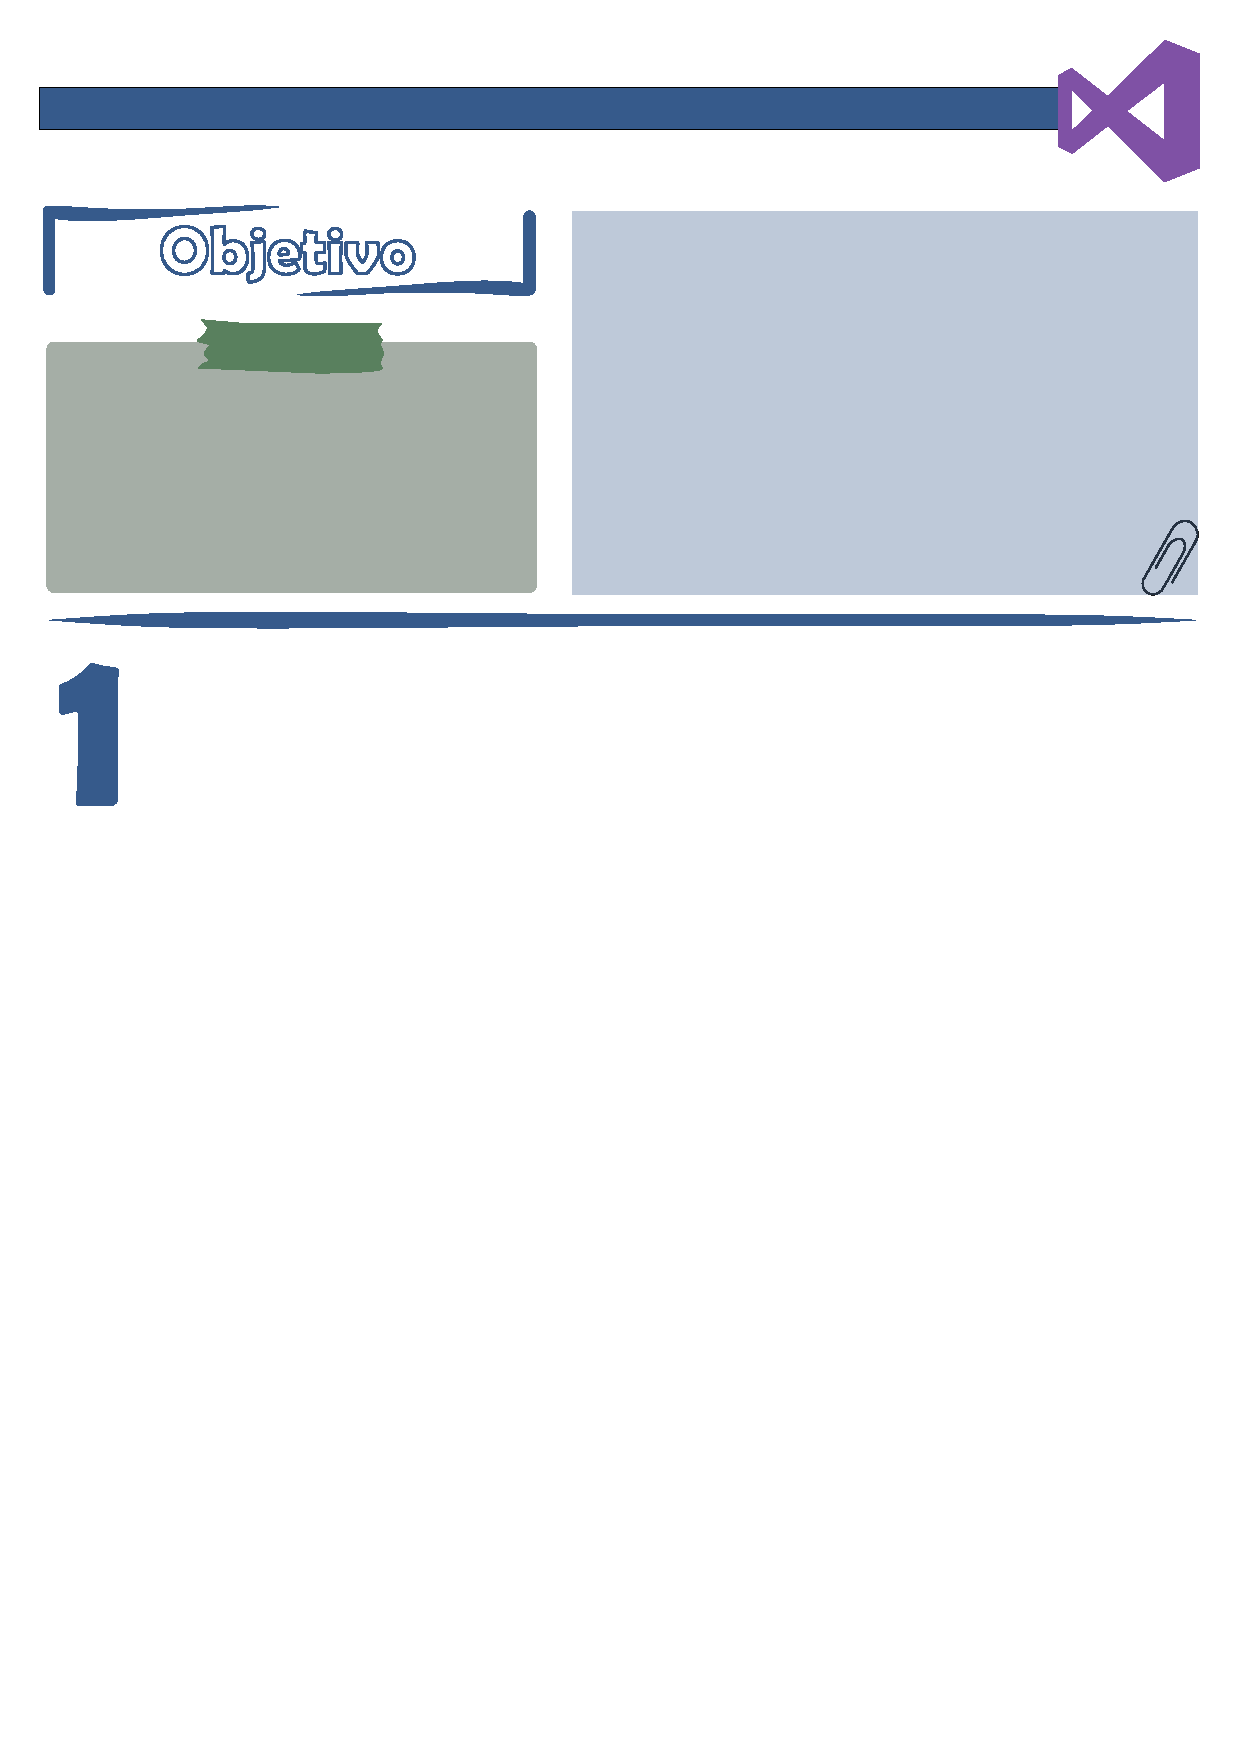
\includegraphics[width = \paperwidth,
		height = \paperheight, keepaspectratio]
		{template2.pdf}}}

\begin{document}
	\fontsize{12}{13.5}\selectfont
	
	\begin{textblock*}{7.2cm}(1.3cm,6.5cm) % {block width} (coords) 
		El propósito del presente documento es explicar la forma de actualizar un proyecto basado en .NET 6 cuyo soporte ha finalizado, a la versión LTS más reciente. Es decir, a .NET 8.
	\end{textblock*}
	
	\begin{textblock*}{9.5cm}(10.3cm,4.3cm) % {block width} (coords) 
		La actualización de un proyecto basado en .NET 6 a .NET 8 consta básicamente de 4 pasos:
		
	\begin{enumerate}
		\item Actualización del TargetFramework en cada uno de los proyectos de la solución.
		\item Actualización de los paquetes Nuget de la solución.
		\item Actualización de la cadena de conexión en el appsettings
	\end{enumerate}
	\end{textblock*}
	
	\begin{textblock*}{17cm}(2.3cm,12.5cm) % {block width} (coords) 
		Cuando creas una nueva aplicación basada en la plantilla de Jabil Core, en Visual Studio, se crean 5 proyectos por defecto contenidos dentro de una misma solución, a saber:
		
		\begin{textblock*}{5cm}(3.3cm,14.1cm) % {block width} (coords)
			\begin{itemize}
				\item Name.Api
				\item Name.DataAccess
				\item Name.Model
				\item Name.Service
				\item Name.Test 
			\end{itemize}
		\end{textblock*}
	\end{textblock*}
	
	\begin{textblock*}{15cm}(5.3cm,13.5cm) % {block width} (coords)
		\begin{figure}[H]
			\centering
			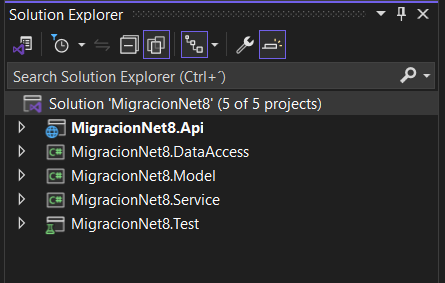
\includegraphics[width=0.5\textwidth]{image1}
			\label{fig:graph1}
		\end{figure}
	\end{textblock*}
	
	\begin{textblock*}{17cm}(2.3cm,18.5cm) % {block width} (coords)
		Para este ejemplo se ha creado un nuevo proyecto usando la plantilla basada en .NET 6 llamado \texttt{MigracionNet8}. El primer paso será actualizar la línea llamada \texttt{TargetFramework} \\
		
		De:
		\begin{lstlisting}[language=HTML]
			<TargetFramework>net6.0</TargetFramework>\end{lstlisting}
		A:
		\begin{lstlisting}[language=HTML]
			<TargetFramework>net8.0</TargetFramework>\end{lstlisting}
			
		Para hacer el cambio, debemos dirigirnos al \textbf{Solution Explorer}, dar clic derecho sobre el proyecto .Api y seleccionar la opción \texttt{Edit Project File}
		\begin{figure}[H]
			\centering
			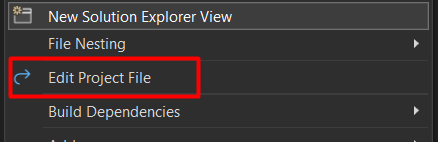
\includegraphics[width=0.5\textwidth]{image3}
			\label{fig:graph2}
		\end{figure}
	\end{textblock*}
	

\end{document}